\documentclass[12pt,a4paper]{article}
\usepackage[utf8]{inputenc}
\usepackage[czech]{babel}
\usepackage[T1]{fontenc}
\usepackage{amsmath}
\usepackage{amsfonts}
\usepackage{amssymb}
\usepackage{graphicx}
\usepackage{epstopdf}
\usepackage{indentfirst}
\setlength{\parindent}{4em} 
\author{Jakub Drápela}
\usepackage{fancyhdr}
\usepackage{siunitx}


%\fontfamily{phs}
%\selectfont

\begin{document}
\pagestyle{empty}

%%nastaveni pisma  
%\fontfamily{phv}
%\selectfont

	\begin{center}

\large

České vysoké učení technické v Praze

\medskip

Elektrotechnická fakulta
\vfill
\vfill
{\LARGE\bfseries Zkoumání vlastností broušeného kamene}


\vspace{15mm}

\vfill
\vfill
\vfill

{\LARGE\bfseries CMP}

\vfill

\begin{tabular}{rl}

Autor: & Jakub Drápela \\
\noalign{\vspace{2mm}}
Studijní obor: & Kybernetika a robotika \\
\noalign{\vspace{2mm}}
Datum vypracování: & \today\\
\end{tabular}

\end{center}

\newpage
\pagestyle{plain}     % zapne obyčejné číslování
\setcounter{page}{1}  % nastaví čítač stránek znovu od jedné  

\tableofcontents
\newpage
\section*{Motivace a myšlenka experimentu}

Jedním z nástrojem ke zkoumání vlastností broušeného kamene je nasvícení jeho povrchu světelným svazkem. Na fasetách broušeného kamene dochází ve zjednodušeném případě k odrazu a lomu světelného svazku. Z toho důvodu se dopadající světelný svazek roztříští na řadu světelných svazků, které z kamene vystupují v různých směrech, s rozdílným zářivým tokem a dalšími typickými vlastnostmi, jako je například polarizace. 
Vystupující světelné svazky lze zachytit na stínítku. Obrazec vzniklý na stínítku jednoznačně charakterizuje broušený kámen. 

Pro tento experiment nasvícení kamene již vznikla řada programů obsahující více či méně věrohodný matematický model. Máme tedy možnost průlet světelného svazku kamenem simulovat. 

V našem případě využíváme program LADOK, který vznikl v Centru strojového vnímání na katedře Kybernetiky ČVUT v Praze. Simulační program LADOK dostatečně přesně určuje matematický model experimentu.

Cestou, jak určit tvar a další typické vlastností kamene, je rozpoznat vystupující paprsky a nalézt takový matematický model, jehož výstup by odpovídal reálné situaci (obrazci na stínítku). 

Problém však tkví v rozpoznání světelných svazků. V tomto případě jde o to ke každému svazku, viditelném na stínítku, přiřadit správnou posloupnost faset kamene, přes které se světelný svazek lomil nebo odrážel. Parametry svazku, které nám pomáhají rozpoznat jeho cestu jsou směr (azimut, elevace), zářivý tok, intenzita, plocha, velikost a směr světelných šmouh, dále nazývaných ocásky, vznikajících při průchodu světelného svazku přes hranu kamene. 

Cílem experimentu je pokusit se nalézt další parametr světelného svazku, jenž by v kombinaci s ostatními parametry pomohl svazek správně rozpoznat. 

Pokusíme se naleznout směr či velikost posunu světelných svazků při rotaci kamene nebo při naklonění zdroje dopadajícího světelného svazku. 

\newpage
\section*{Teoretický rozbor problému}

Rotace kamene kolem osy způsobí změnu vlastností vystupujících světelných svazků (směru, zářivého toku, intenzity, vlastnosti ocásků atd.). Za určitých okolností může světelný svazek zcela vymizet. Tato situace nastává například při lomu světelného svazku z kamene do okolí. Když vlivem rotace překročíme kritický úhel, nedochází k vylomení světelného svazku, ale k totálnímu odrazu na fasetě. Světelný svazek také postupně zmizí při posunu světelného svazku mimo fasetu, a to jak při odrazu, tak při lomu. Ze stejných důvodů, proč mohou světelné svazky vymizet, mohou naopak vzniknout svazky nové.

Uvažujeme zjednodušenou situaci. Světelný svazek nahradíme světelným paprskem ležícím v jeho pomyslném těžišti. 

Světelný paprsek necháme dopadat na zrcadlo pod úhlem $\varphi_1$ a od nějž se odráží podle známého zákonu odrazu pod úhlem $\varphi_1$. Při vychýlení světelného paprsku o úhel $ \delta $ v kladném směru úhlu $\varphi_1$ je odražený úhel $\varphi_1 + \delta$. Odražený paprsek se otočí o úhel $ \delta $.

\begin{figure}[h!]
\begin{center}
\scalebox{1}{ \input{xfig/odraz2.pstex_t}}
\end{center}
\caption{Odraz laseru od zrcadla. Změna úhlu dopadajícího světelného paprsku vyvolá stejně velkou změnu úhlu odraženého paprsku.}
\label{fig:odraz laser}
\end{figure}

Jiná situace nastává při rotaci zrcadla kolem osy o úhel $\alpha$ v záporném směru. Světelný paprsek dopadá na zrcadlo pod úhlem $\varphi_1 + \alpha$. Odráží se pod úhlem $\varphi_1+\alpha$, ale vzhledem k tomu, že vstupní parsek je ve stejné pozici, se výstupní paprsek otočí o úhel  $2\alpha$. 


Důsledkem toho dostaneme identické výsledky experimentu při rotaci kamene, jako při natočení světelného zdroje o dvojnásobný úhel v opačném směru. Dále budeme tedy uvažovat pouze rotaci kamene. 

\newpage
\begin{figure}[h!]
\begin{center}
\scalebox{1}{ \input{xfig/odraz.pstex_t}}
\end{center}
\caption{Odraz laseru od rotujícího zrcadla. Rotace zrcadla vyvolá dvojnásobnou změnu velikosti úhlu odraženého paprsku.}
\label{fig:odraz zrcadlo}
\end{figure}

Pokud by docházelo pouze k odrážení od zrcadel v dvojrozměrné rovině, tak by naše zkoumání postrádalo smysl. Výstupní parsek by se vždy otočil o dvojnásobek úhlu rotace kamene a to ve stejném směru. 

S uvažováním materiálu kamene s konstantním indexem lomu $ n_1>1 $ a okolí s indexem lomu $ n_2 = 1 $ se situace dramaticky mění. Vezměme si příklad lomu světelného paprsku z kamene přes rovinnou fasetu. Úhel dopadajícího paprsku na fasetu označme $\alpha_1$ a úhel lomeného svazku $\alpha_2$, pak můžeme podle Snellova zákonu psát

\begin{center}
$n_1\,\sin(\alpha_1) = n_2\,\sin(\alpha_2) = \sin(\alpha_2)\,.$
\end{center}

\begin{figure}[h!]
\begin{center}
\scalebox{.9}{ \input{xfig/index.pstex_t}}
\end{center}
\caption{Tři případy, které mohou nastat při dopadu světelného paprsku na fasetu. Zleva lom paprsku z kamene, dopad pod kritickým úhlem a totální odraz.}
\label{fig:lom ven }
\end{figure}

Zkoumejme změnu výstupního úhlu $\alpha_2$ na změně úhlu $\alpha_1$. Nejprve si vyjádříme úhel $\alpha_2$ následně zderivujeme podle $\alpha_1$. 

\begin{center}
$\alpha_2 = \arcsin(n_1\,\sin\alpha_1) \implies \frac{\mathrm{d}\alpha_2}{\mathrm{d}\alpha_1}= \frac{n_1\,\cos\alpha_2}{\sqrt{1-n_1^2\,\sin^2\alpha_2}}$
\end{center}

Pokud se dostáváme ke kritickému úhlu $\alpha_k$, kdy dochází k totálnímu odrazu, potom

\begin{center}
 $	\sin\alpha_2 = 1 \implies \sin\alpha_1 = \frac{1}{n_1}\,. $
\end{center}

Změnu výstupního úhlu $\alpha_2$ a vypočtením limity v okolí kritického úhlu pro $ n_1>1$ dostaneme 

\begin{eqnarray}
\lim_{n \to \alpha_k}\frac{\mathrm{d}\alpha_2}{\mathrm{d}\alpha_1} = \frac{n_1\,\cos(\arcsin\frac{1}{n_1})}{\sqrt{1-n_1^2\,\frac{1}{n_1^2}}} \to \infty\,.
\label{eq:zmena velikosti posunu}  
\end{eqnarray}

Velikost změny posunu světelného svazku tedy může být teoreticky libovolně větší než je index lomu $n_1$, což je minimum grafu na obr. \ref{fig:derivace uhlu}. 

\begin{figure}
\begin{center}
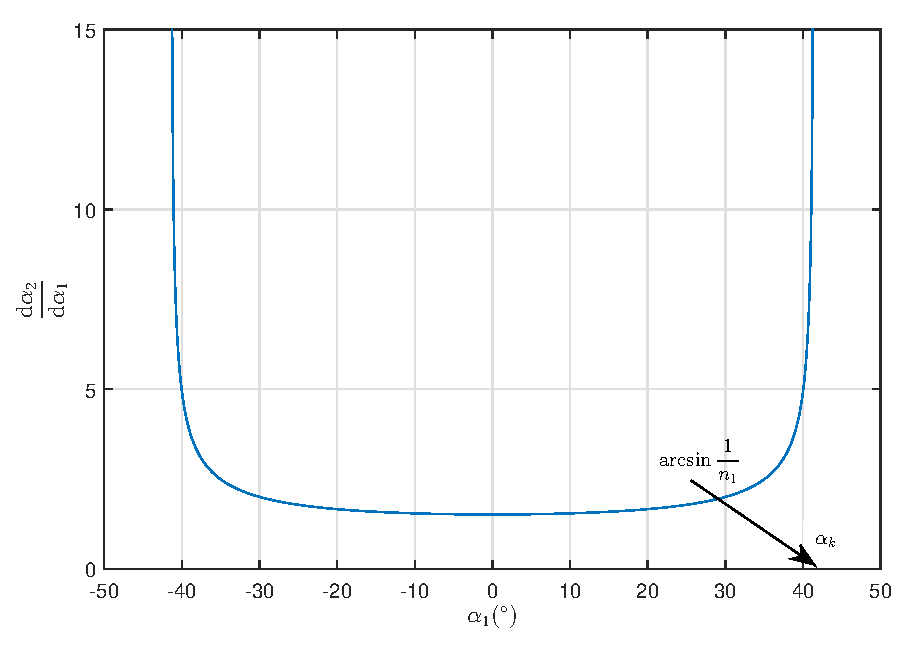
\includegraphics[width = 10cm]{figures/derivace.eps}
\end{center}
\caption{Závislost lomeného úhlu na dopadajícím úhlu. Pro kritický úhel roste k nekonečnu. Graf funkce popsané vzorcem \ref{eq:zmena velikosti posunu}.}
\label{fig:derivace uhlu}
\end{figure}
\newpage


\section*{Modelování pohybu v LADOKU}

V programu pro simulaci průchodu světelného paprsku konvexním objektem jsme provedli experiment s rotací broušeného kamene. Pro svoji jednoduchost jsme vybrali kámen ve tvaru šatonové růže s 12 bočními fasetami, tabulkou a spodkem ideálního tvaru. Obchodně jej lze nalézt pod názvem VIVA12.

Kámen jsme rotovali kolem souřadné soustavy umístěné v těžišti spodku kamene o úhel konstantní velikosti. Rotací kamene okolo osy $z$ dostaneme pouze soustředné kružnice. Pří tomto experimentu jsme kámen rotovali okolo osy $x$ a dostali výsledek z obrázku \ref{fig:relativni pohyb graf}.

Z praktického hlediska nás zajímají svazky, které lze detekovat. K detekci se v naší laboratoři používá kamera. Ve snímku získaném kamerou lze rozeznat pouze svazky se zářivým tokem, který přebije okolní rozptyl ostatních světelných svazků. Navíc záleží také na kvalitě kamery. Svazky s velmi malým zářivým tokem jsou zastíněny a ztraceny v okolním šumu, proto je není zapotřebí uvažovat. Takové svazky jsme z obrázku \ref{fig:relativni pohyb graf} vyloučili. 

% obrazek pohybu jednotlivych stop 
\begin{figure}[h!]
\begin{center}
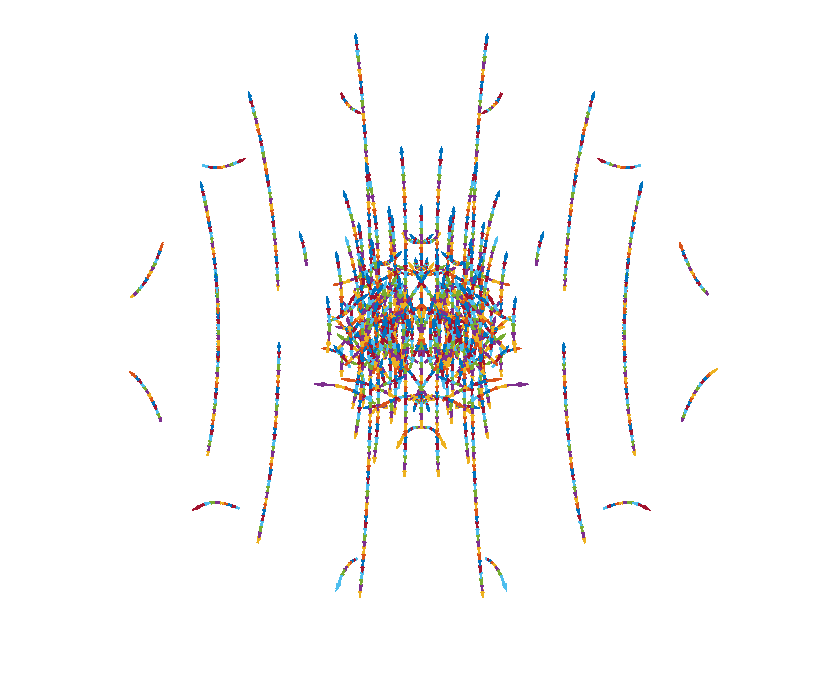
\includegraphics[width = 10cm]{figures/viva12_bigflux.eps}
\end{center}
\caption{Dráhy posunu jednotlivých světelných svazků vycházejících z kamene VIVA12 získané simulačním  LADOK. Zobrazeny jsou svazky vycházející v horní polorovině kamene. }

\label{fig:relativni pohyb graf}
\end{figure}

\newpage
Pro lepší představu o posunu jednotlivých svazků nám může být užitečný kruhový histogram znázorňující směr jejich posunu (obr. \ref{fig:relativni pohyb graf}). Na něm vidíme, že obrovská část se pohybuje ve směru rotace kamene. Podstatná většina svazků se posouvá ve směru rotace kamene, což ovšem není příliš nápomocné při jejich rozeznávání.

Existují však svazky, které jsou svým pohybem charakteristické a lze je tedy oddělit od ostatních. Kritériem pro rozeznání svazků nemusí být pouze směr posunu, ale jak vidíme na obr. \ref{fig:relativni pohyb graf} i velikost posunu. V neposlední řadě přichází v úvahu i změna zářivého toku svazků, změna velikosti ocásků a další. 

\begin{figure}[h!]
\begin{center}
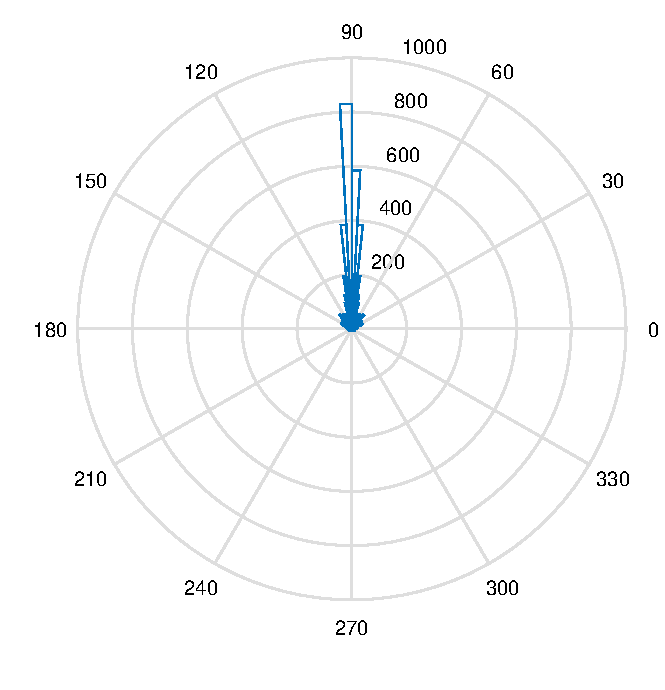
\includegraphics[width = 7cm]{figures/kruhovy_histogram.eps}
\end{center}
\caption{Kruhový histogram směru posunu jednotlivých světelných svazků kamene VIVA12 z obrázku \ref{fig:relativni pohyb graf}. Většina stop se posunuje ve směru rotace kamene.}
\label{fig:kruhovy histogram}
\end{figure}

Vykresleme si histogram (obr. \ref{fig:histogram relativni pohyb } vlevo) velikosti posunu svazku. Z něj je patrné, že řada svazků se posune o více než dvojnásobek, což potvrzuje teorii o relativní změně velikosti z rovnice \ref{eq:zmena velikosti posunu}. 

\begin{figure}[h!]
 \begin{center}
 

   \begin{minipage}[c]{0.45\textwidth}
     \centering 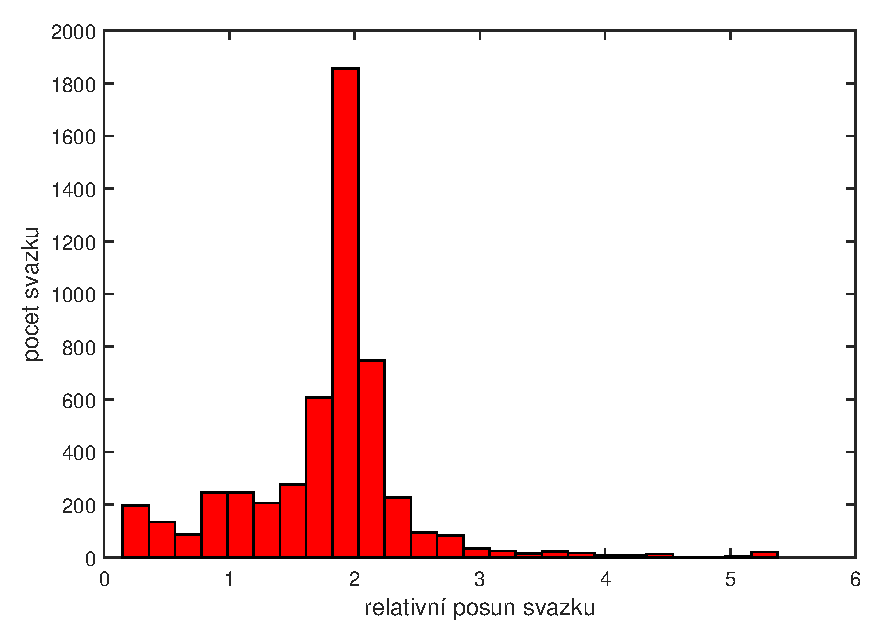
\includegraphics[height =4.5cm]{figures/relative.eps} 
   \end{minipage}
   \begin{minipage}[c]{0.45\textwidth}
     \centering 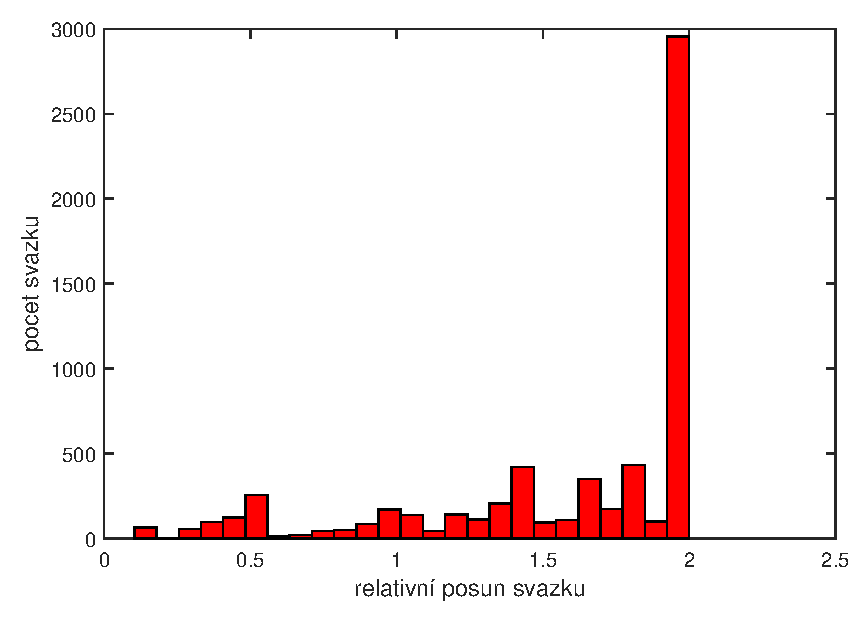
\includegraphics[height =4.5cm]{figures/relative_index1.eps} 
   \end{minipage}
 \end{center}
\caption{Vlevo histogram velikosti posunu světelných svazků kamene VIVA12 z obrázku \ref{fig:relativni pohyb graf}. Vlivem lomu je relativní posun v mnoha případech vetší než 2. V okolí kritického úhlu roste k nekonečnu. Pokud ztotožníme indexy lomu kamene a okolí, tak relativní posun nebude vetší než 2. To lze vidět na histogramu vpravo.}

\label{fig:histogram relativni pohyb }

\end{figure}

Pokud vezmeme teoreticky kámen se stejným indexem lomu, jako je okolí, neměl by se v kameni lom ojevovat. Potom relativní by se změna posunu výstupního svazku větší než 2, způsobená právě rozdílným indexem lomu,  neměla vůbec objevovat. Pro potvrzení této teorie jsme provedli stejnou simulaci jako v předchozím případě. Indexy lomu jsme ztotožnili a výsledek simulace ukázal, že právě relativní posuny výstupního svazku větší než 2 vymizely. To nám dokládá zhotovený histogram (obr. \ref{fig:histogram relativni pohyb } vpravo)



\newpage
\begin{figure}[h!]
\begin{center}
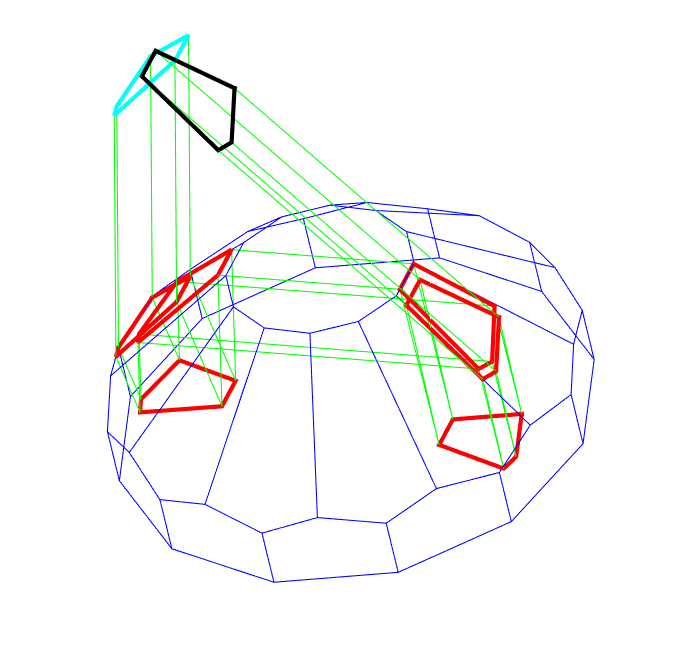
\includegraphics[width = 7.5cm]{figures/odraz.eps}
\end{center}
\caption{Průlet světelného svazku kamenem VIVA12. Příklad s velkou změnou vystupujícího úhlu. Dopad světelného svazku na fasetu kamene je znázorněn hranolem s modrým okrajem. Svazek vystupující z kamene je hranol s černým okrajem. Svazek kamenem putuje následovně: 1. lom do kamene, 2. odraz od spodku, 3. odraz od fasety, 4. odraz od fasety na protější straně, 5. odraz od spodku, 6. dopad na fasetu pod úhlem blízkým kritickému úhlu a vylomení z kamene.}

\label{fig:odrazy v kamenu}
\end{figure}
\newpage

Vesměs konstantní směrovost posunu svazků u kamene VIVA12 zmenšuje význam příspěvku této vlastnosti k lepšímu rozpoznání světelných stop. Pokud ovšem provedeme stejný experiment na broušeném kameni jiného tvaru, dostaneme rozdílný výsledek. Například u šatonu, svým tvarem složitějším než VIVA12, je směr posunu svazků rozmanitější. Velká část z nich se samozřejmě pohybuje ve směru rotace kamene. Jak ale vidíme z kruhového histogramu (obr. \ref{fig:kruhovy histogram saton}), lze rozlišovat i velké množství stop pohybujících se např. pod úhlem $45^\circ$. U šatonu tedy může směr pohybu svazků nemalou měrou pomoci v jejich rozpoznání. 

\begin{figure}[h!]
\begin{center}
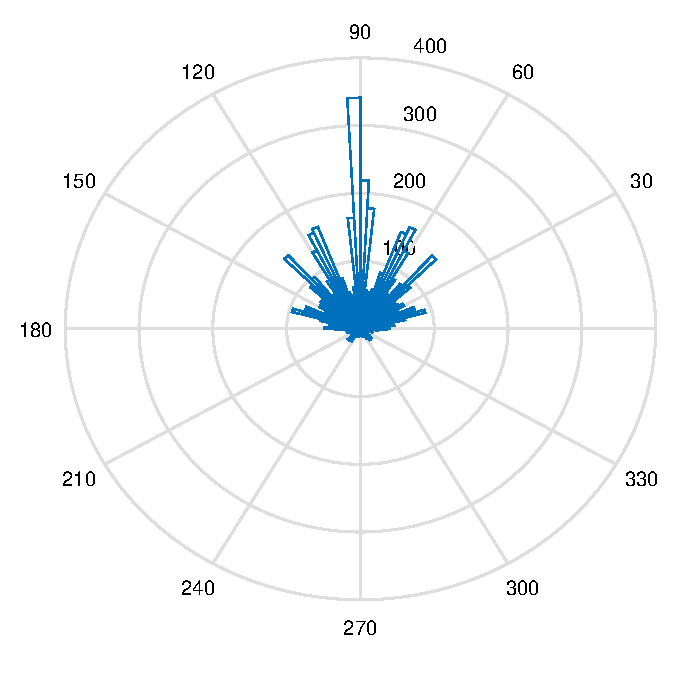
\includegraphics[width = 7cm]{figures/saton_smer.eps}
\end{center}
\caption{Kruhový histogram směru posunu jednotlivých světelných svazků u šatonu. Svazky se pohybují různými směry, kterými lze svazky charakterizovat.}

\label{fig:kruhovy histogram saton}
\end{figure}

\newpage


\section*{Experiment na reálném kameni}
Od počítačové simulace přejdeme k experimentu s reálným kamenem. Cílem experimentu je zjistit, zda výsledky, které naměříme lze porovnat s výsledky získanými pomocí matematického modelu. 

Zdrojem koherentního světelného svazku je laser. Laserové záření dopadá na broušený kámen, kde se roztříští na mnoho menších svazků. Svazky opouštějící kámen v horní polorovině jsou zachyceny na kulovém stínítku a na něm vznikne jedinečný světelný obrazec. Tento obrazec snímá kamera a vzniká digitální obraz. V obraze detekujeme laserové stopy na stínítku a z nich správnou transformací určujeme vlastnosti světelných svazků vystupujících z kamene. 

Zkoumaný kámen jsme vybrali ve tvaru šatonové růže s 12 bočními fasetami, tedy opět VIVA12 jako v počítačové simulaci. Jedná se o kámen červené barvy s označením Hyacint. Průměr kamene je takový, aby na celý jeho povrch dopadalo laserové záření. V našem případě \SI{2.8}{\milli\metre}. 
\begin{figure}[h!]
 \begin{center}
 

   \begin{minipage}[c]{0.69\textwidth}
     \centering 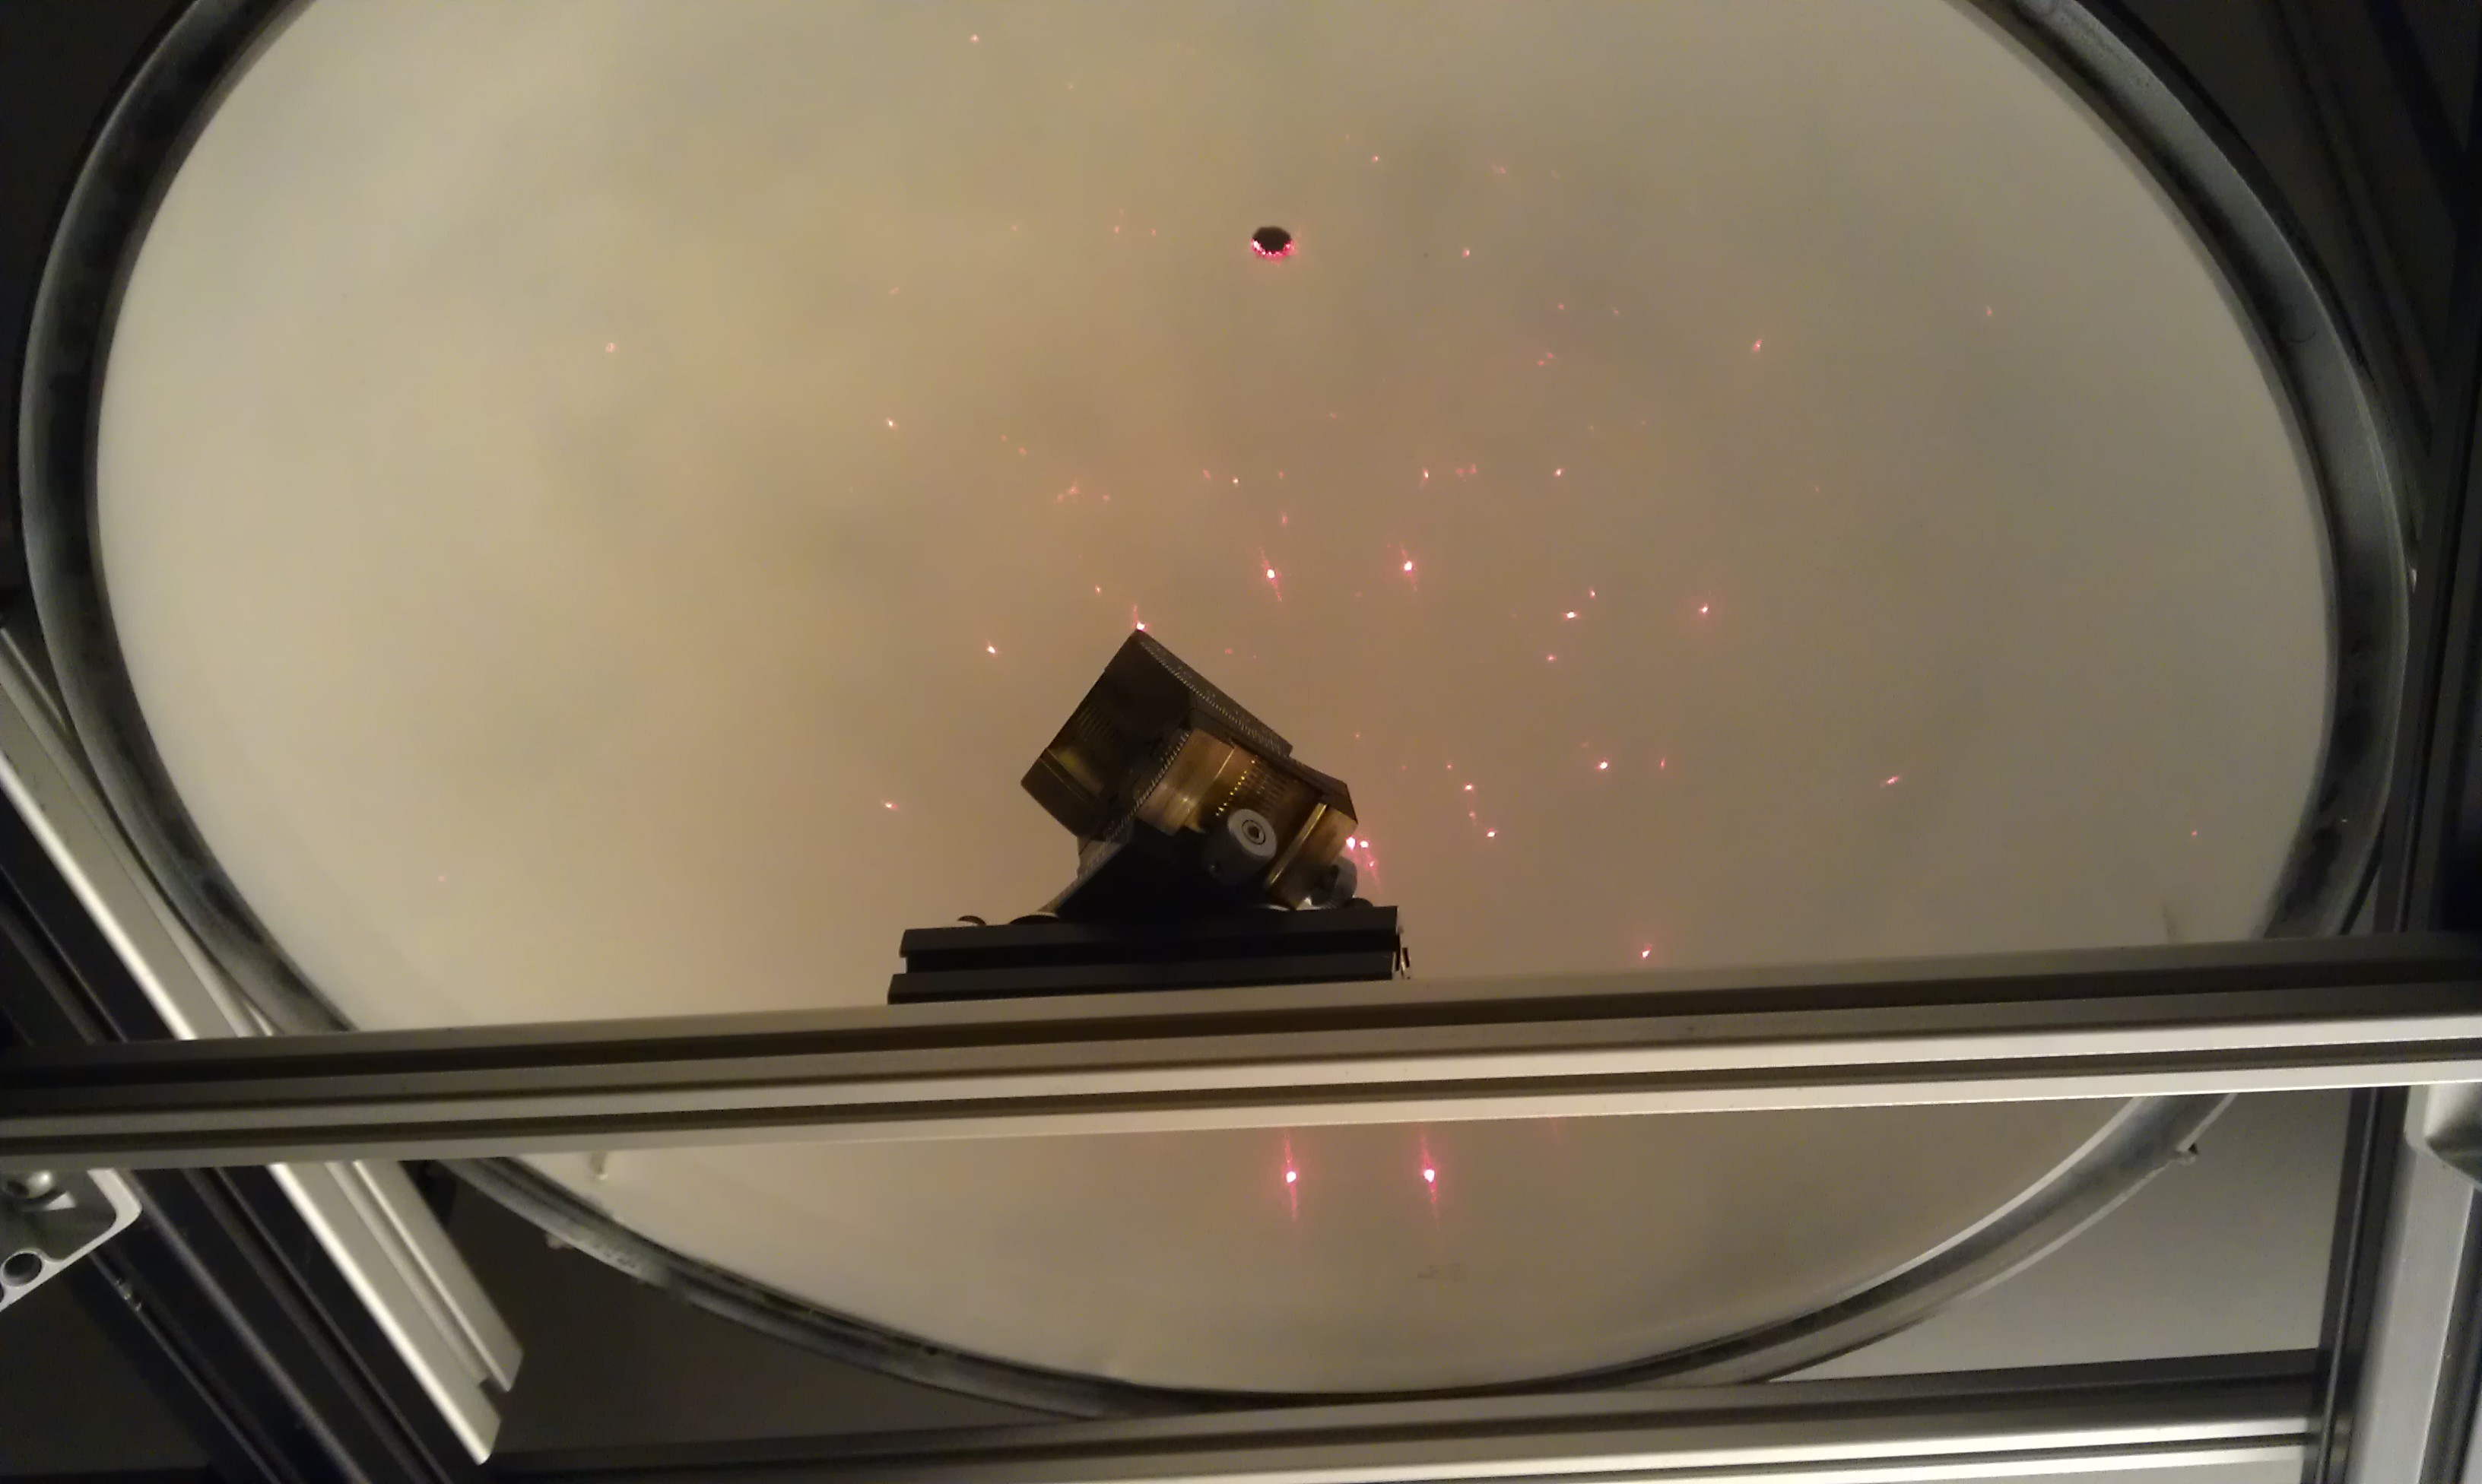
\includegraphics[ height =5cm]{img/stolek} 
   \end{minipage}
   \begin{minipage}[c]{0.29\textwidth}
     \centering 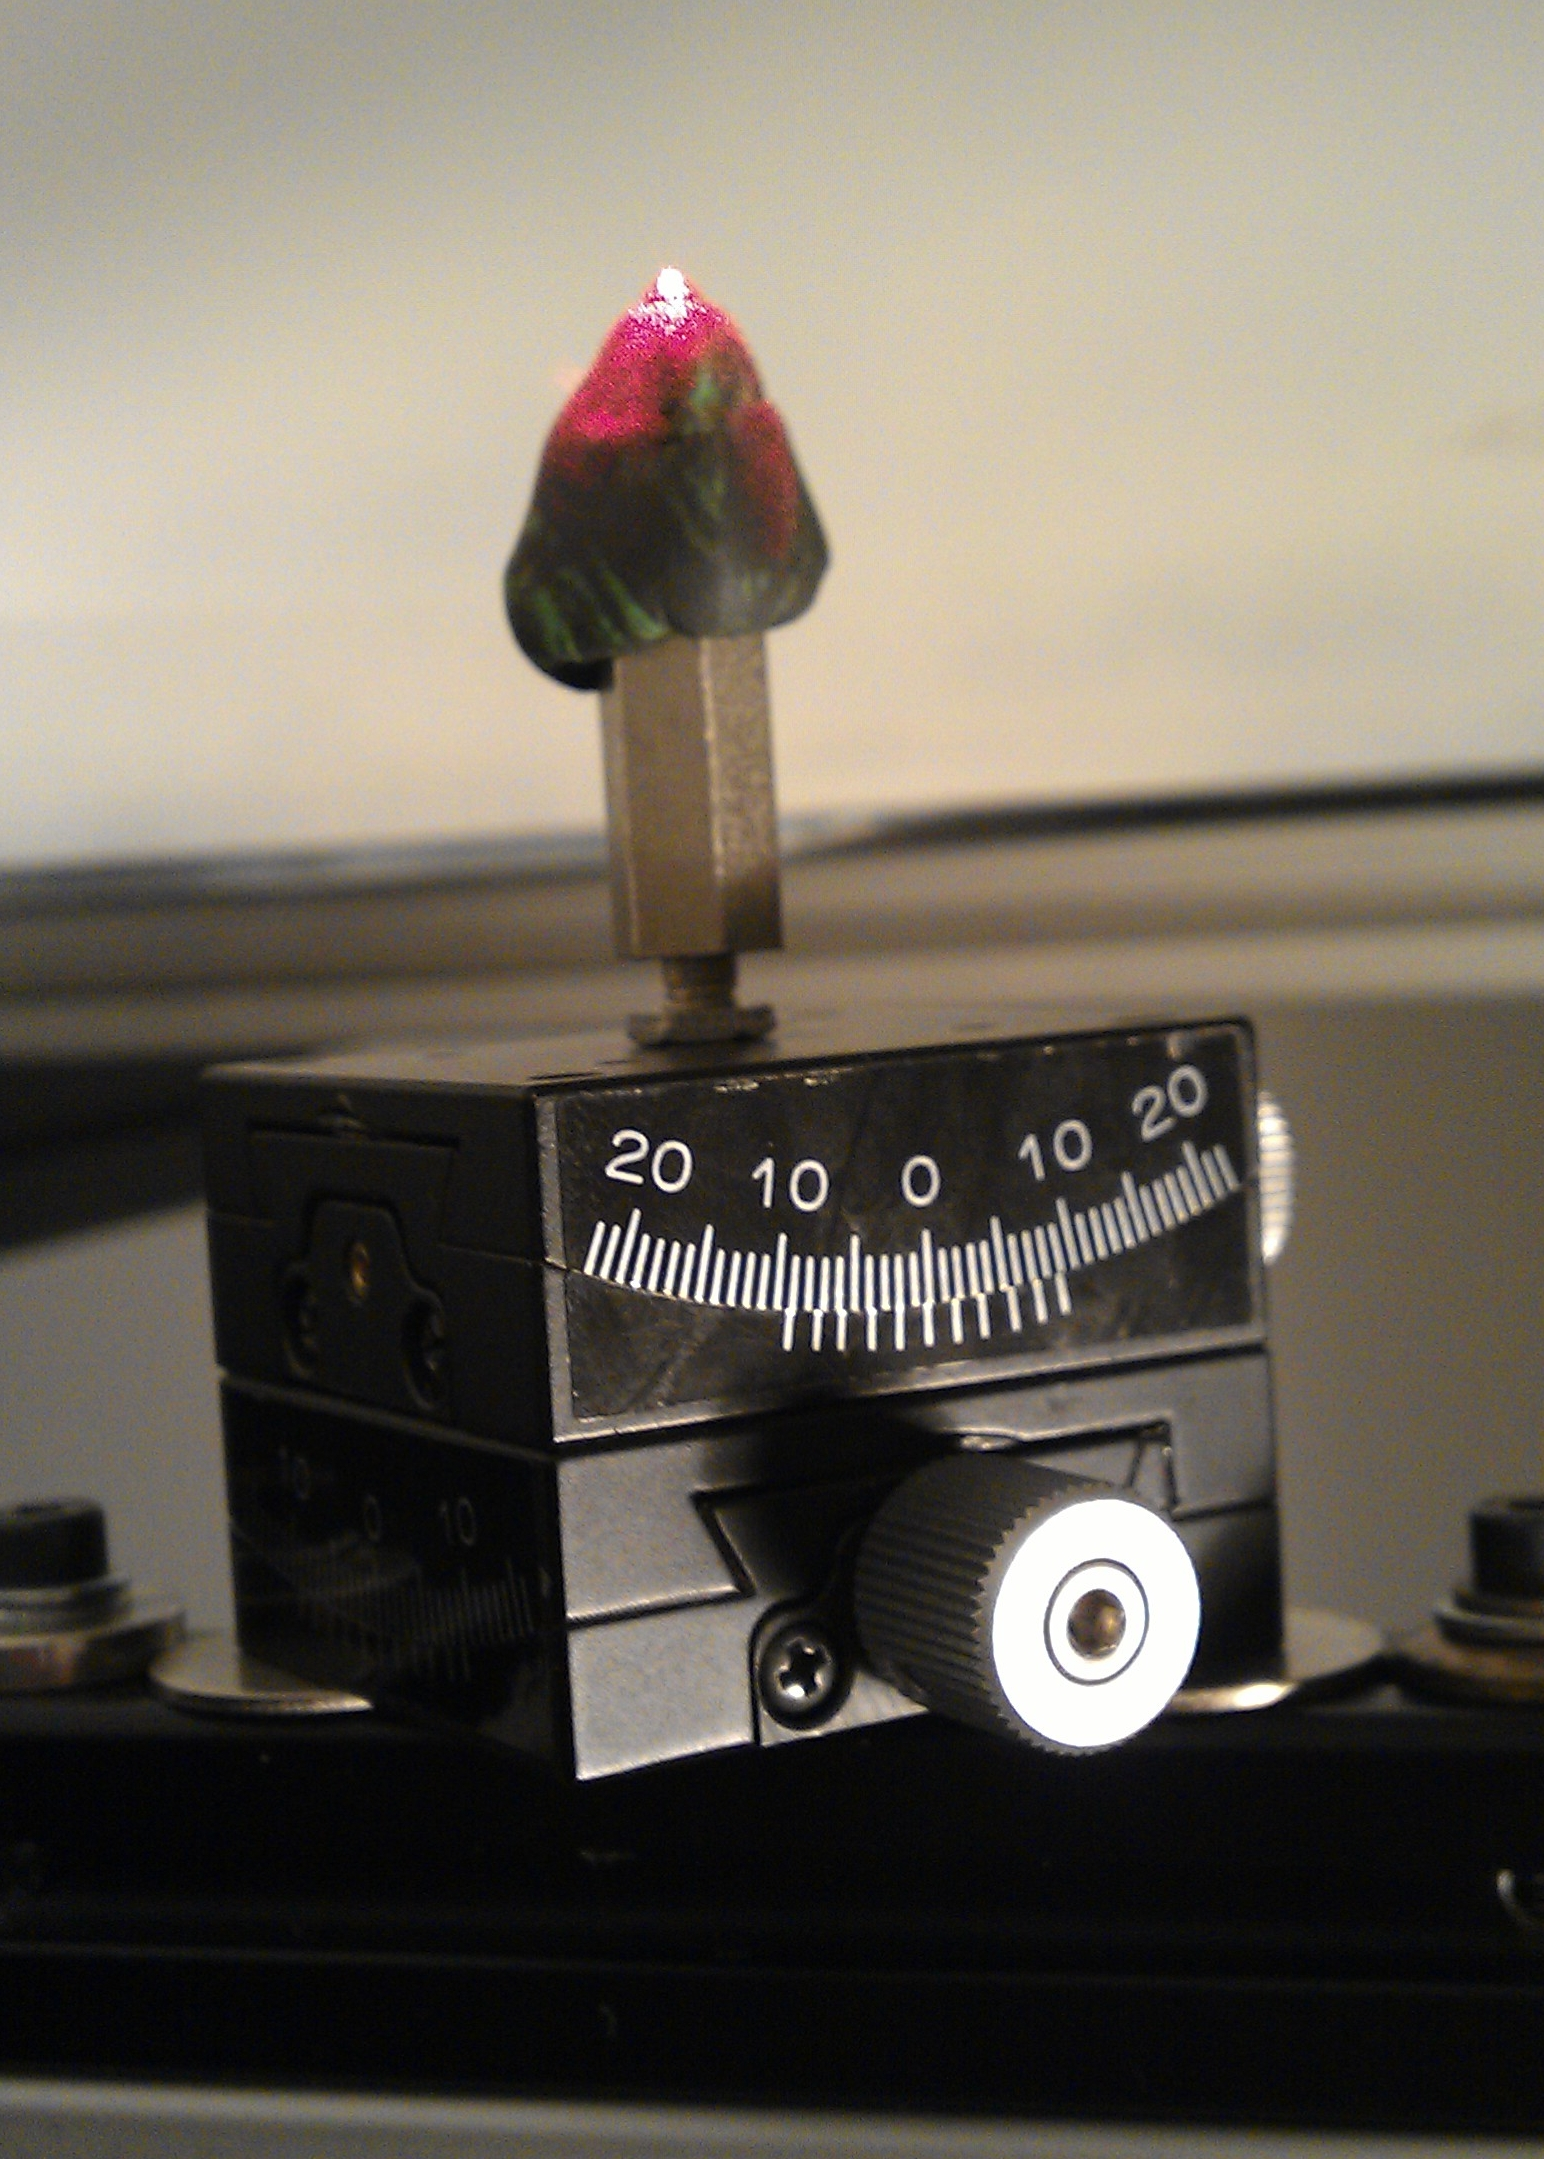
\includegraphics[height =5cm]{img/stolek-detail22} 
   \end{minipage}
 \end{center}

   \caption{Pohybová část měřicí soustavy. Laserové záření proniká otvorem na vrcholku bílé polokoule. Koherentní záření dopadá na kámen VIVA12 připevněný plastelínou na vrcholku prodloužení dvojice goniometrů. Goniometry je možné polohovat, kámen rotovat ve dvou osách a posouvat světelný obrazec po stínítku.}
   \label{fig:merici soustava}
 \end{figure}
 
 Kamenem jsme rotovali kolem tak, abychom mohli výsledky z reálného experimentu vizuálně porovnat s výsledky simulace. Při každém kroku jsme kámen rotovali o $\sqrt{2}$ stupně. Celkem jsme naměřili výsledky pro 41 pozic kaneme symetricky rozdělených kolem vrcholu půlkulového stínítka. Mezi obrazy lišícími se jedním krokem rotace jsme našli korespondující body. Při procesu hledání korespondencí vznikají chybná přiřazení. Je jich však tak málo, že při vizuálním porovnání nemají velký vliv. 
 
Korespondující body ze všech naměřených snímků jsme spojili do jednoho, přičemž jsme jejich pohyb znázornili vektory. Na obrázcích \ref{fig:graf posunu porovnani}, \ref{fig:relativni posun porovnani} je vidět porovnání výsledku se simulovanými daty.  

\begin{figure}[h!]
 \begin{center}
 

   \begin{minipage}[c]{0.49\textwidth}
     \centering 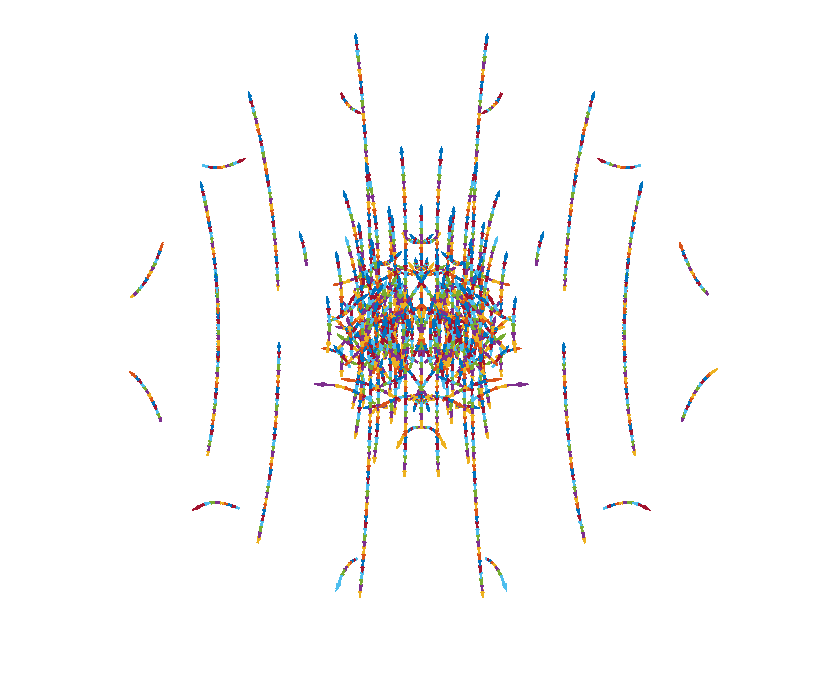
\includegraphics[height =5cm]{figures/viva12_bigflux} 
   \end{minipage}
   \begin{minipage}[c]{0.49\textwidth}
     \centering 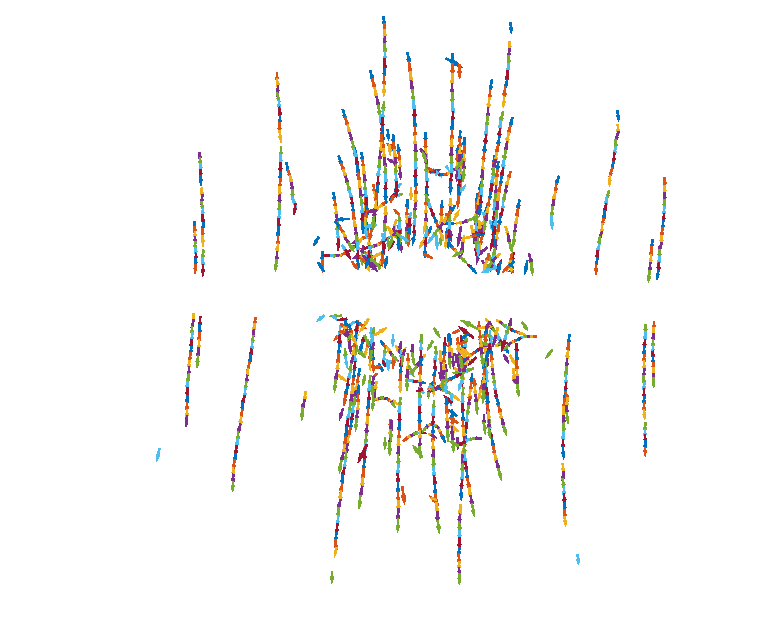
\includegraphics[height =5cm]{figures/real_all} 
   \end{minipage}
 \end{center}

   \caption{Porovnání výsledku z počítačové simulace s výsledky z reálného experimentu. Vlevo máme výsledky posunu stop kamene  vypočtené pomocí matematického modelu kamene. Obrázek je totožný s obr. \ref{fig:relativni pohyb graf}. Obrázek vpravo znázorňuje výsledky z experimentu s reálným kamenem. Data nejsou úplná, neboť z pohledu kamery část půlkulového stínítka zakrývá konstrukce pro připevnění goniometrů. Oba výsledky jsou si vizuálně podobné. Blízko středu obrázku se objevují typické oblouky spojené se svazky podobného typu, jako na obrázku \ref{fig:odrazy v kamenu}, kde je znázorněna jeho trasa kamenem.}
   \label{fig:graf posunu porovnani}
 \end{figure}
 
\begin{figure}[h!]
 \begin{center}
 

   \begin{minipage}[c]{0.45\textwidth}
     \centering 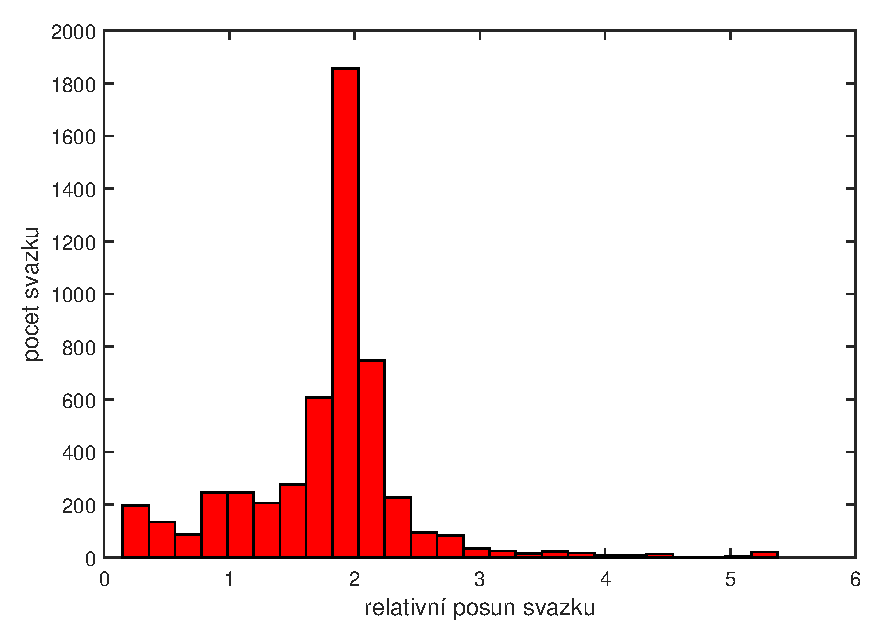
\includegraphics[height =4.5cm]{figures/relative} 
   \end{minipage}
   \begin{minipage}[c]{0.45\textwidth}
     \centering 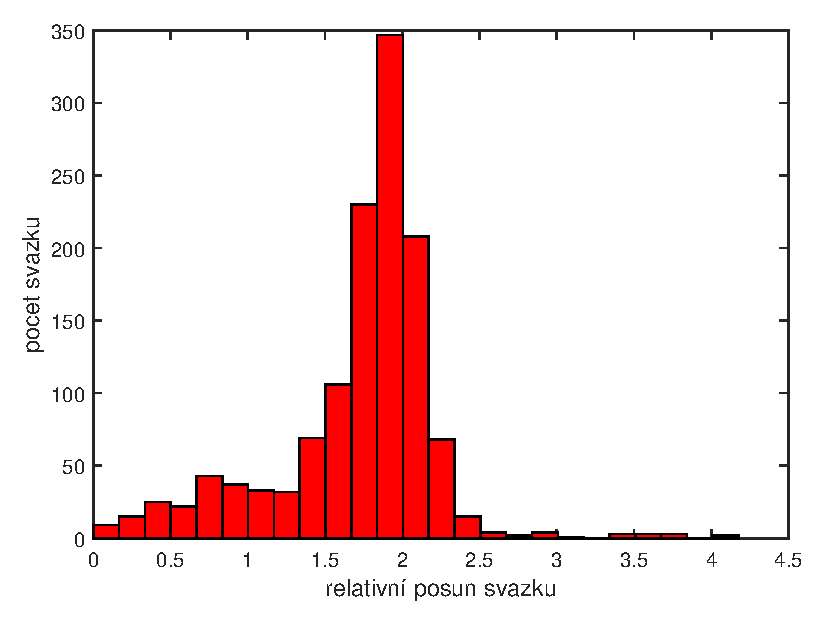
\includegraphics[height =4.5cm]{figures/real_relative} 
   \end{minipage}
 \end{center}

   \caption{Porovnání výsledku z počítačové simulace s výsledky z reálného experimentu - velikost posunu. Vlevo máme histogram velikosti posunu stop kamene  vypočtené pomocí matematického modelu kamene. Obrázek je totožný s obr. \ref{fig:histogram relativni pohyb } vlevo. Obrázek vpravo znázorňuje histogram velikosti posunu stop z experimentu s reálným kamenem. Podobnost je i zde patrná.}
  \label{fig:relativni posun porovnani}
 \end{figure}

  
%\clearpage

\end{document}
